% ============================================================================
% HOG Features (Image processing, 12 points)
% Generated by assignment2/src/3_HOG.py. All numbers below come from its output.
% Requires: graphicx, float, booktabs (same preamble as Assignment 1).
% Figures: upload assignment2/rapport/figurer/hog_*.png to figurer/ in Overleaf.
% ============================================================================

\section{HOG Features}

\textbf{1.}
We compute HOG features with \texttt{skimage.feature.hog} (script \texttt{3\_HOG.py}). The image is converted to grayscale in $[0,1]$. HOG then computes the gradient of every pixel with the centred filter $[-1,0,1]$, giving the magnitude $|G|=\sqrt{G_x^2+G_y^2}$ and the unsigned orientation $\theta \in [0^\circ,180^\circ)$. The image is split into cells, and each pixel votes for the orientation bin of its gradient, weighted by $|G|$. Groups of neighbouring cells, called blocks, are concatenated and normalised with L2-Hys: L2 normalisation, clipping at 0.2, then L2 normalisation again. The blocks overlap with a stride of one cell. We use the settings from Dalal and Triggs as the baseline: 9 bins, $8\times8$ pixel cells and $2\times2$ cell blocks. For the gradient image we compute $G_x$ and $G_y$ ourselves with the same filter, since \texttt{hog} only returns the descriptor and the visualisation. Throughout the section, $0^\circ$ is a horizontal gradient, which means a vertical edge, and $90^\circ$ is a vertical gradient, which means a horizontal edge.

\textbf{2.}
HOG may be applied to any images, so we combine one image from our dataset with three standard images from \texttt{skimage.data}, chosen to range from simple to complex (Figure~\ref{fig:hog-overview}):
\begin{itemize}
    \item \textbf{Horse}: a black silhouette on a white background, the simplest possible scene.
    \item \textbf{Heatmap}: participant 0 on slide \texttt{hm20}, i.e.\ text on a white slide with fixation blobs.
    \item \textbf{Camera}: a grayscale photograph with one clear subject and a textured lawn.
    \item \textbf{Astronaut}: a colour photograph with many objects, a face and fine texture.
\end{itemize}
All images are cropped to a square and resized to $256\times256$ pixels, so that every descriptor has the same length and can be compared element by element. With the baseline settings this gives $31\times31$ blocks of $2\cdot2\cdot9=36$ values, i.e.\ 34,596 features per image. At full resolution one heatmap ($960\times540$) would give 282,744 features. For the heatmap we keep the left $540\times540$ region, where the text and fixations are.

\textbf{3.}
Figure~\ref{fig:hog-overview} shows each image, the gradient magnitude, the gradient direction as colour, and the HOG visualisation, where each cell is drawn as a star of lines along the edges, one per bin, with brightness proportional to the bin value. Figure~\ref{fig:hog-zoom} zooms in on the camera image to make the individual cell histograms visible.

\begin{figure}[H]
    \centering
    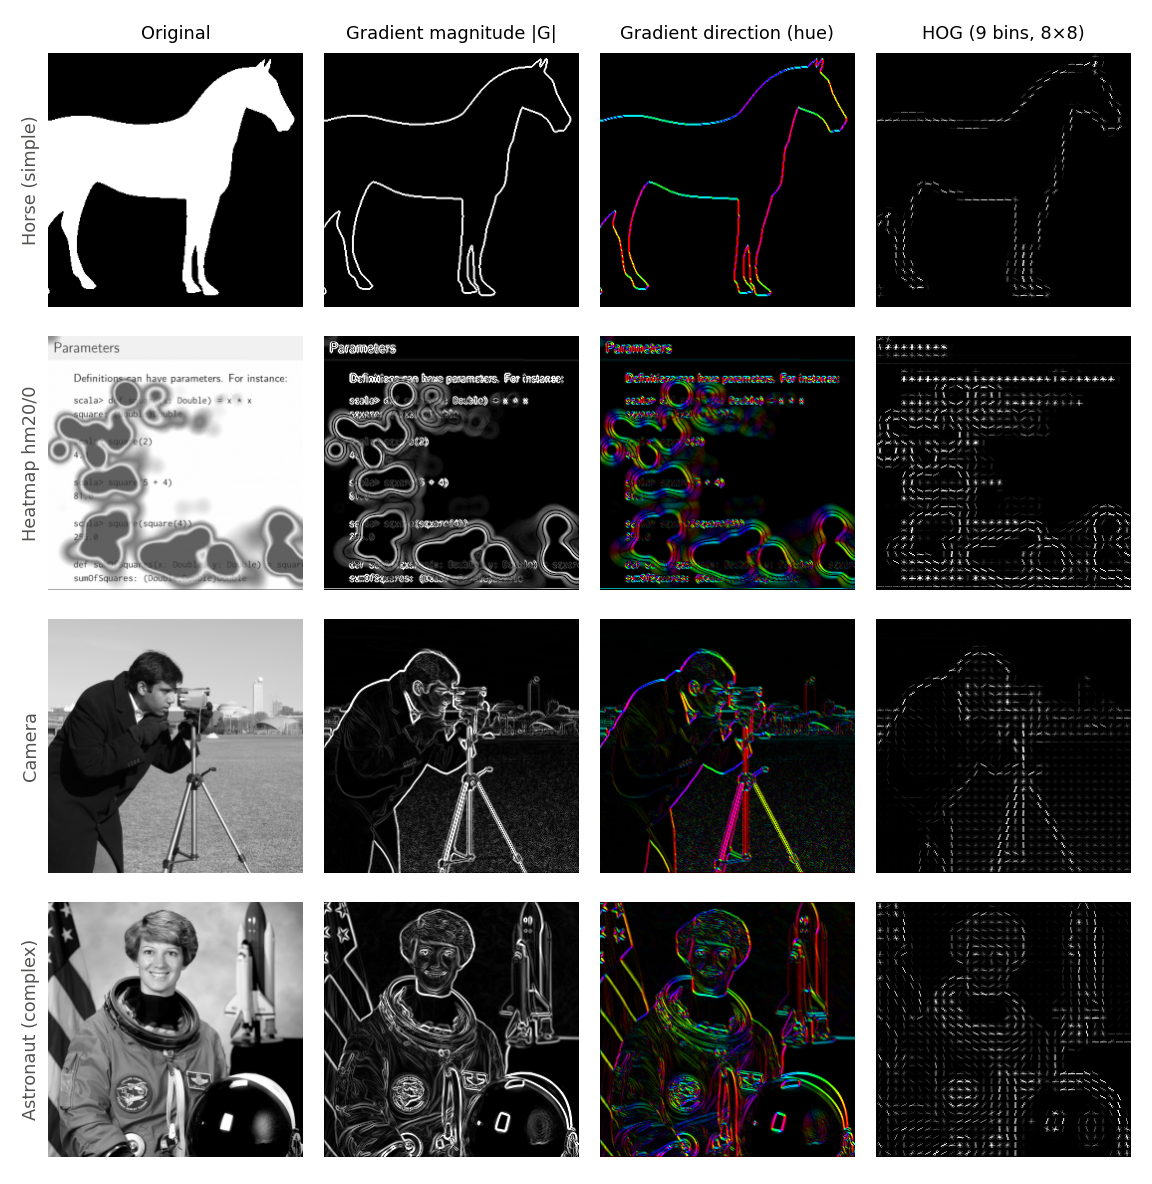
\includegraphics[width=\textwidth]{figurer/hog_oversikt.png}
    \caption{Original, gradient magnitude, gradient direction (hue, $0^\circ$--$180^\circ$, brightness $=|G|$) and HOG image with 9 bins, $8\times8$ cells and $2\times2$ blocks.}
    \label{fig:hog-overview}
\end{figure}

\begin{figure}[H]
    \centering
    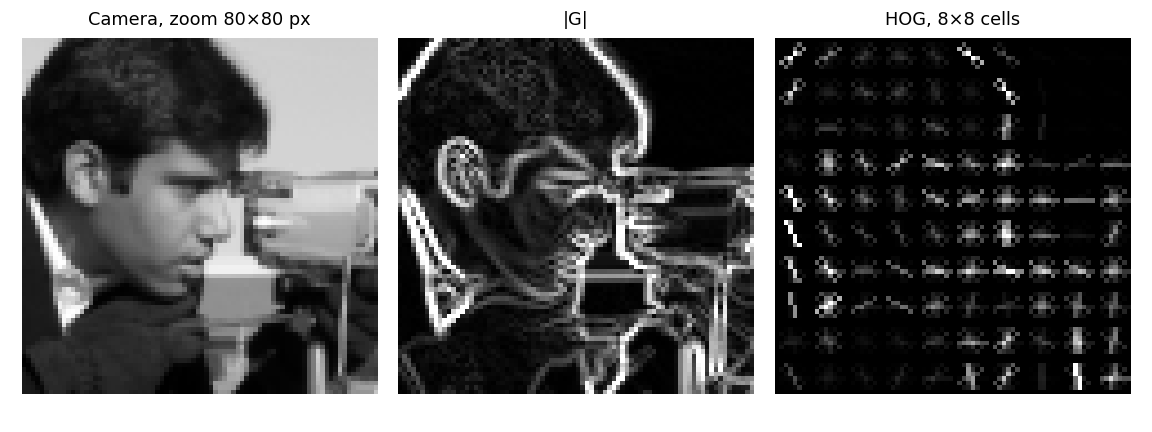
\includegraphics[width=\textwidth]{figurer/hog_zoom.png}
    \caption{An $80\times80$ pixel region of the camera image. Each $8\times8$ cell becomes one histogram. Straight edges such as the cheek and the camera give one dominant line, and hair and textured regions give weak lines in all directions.}
    \label{fig:hog-zoom}
\end{figure}

The gradient image shows where the image changes, and the HOG image shows how the changes are oriented within each cell. The horse is reduced to its outline, and 82\% of its cells are flat (mean $|G|<0.01$) and contribute nothing. The astronaut has only 14\% flat cells, and the camera image 32\%, mostly in the sky. The heatmap reveals a property of our dataset: after conversion to grayscale, the red centre and the green and blue edges of each fixation blob get different intensities, so every blob gets a double ring of gradients. HOG therefore describes a blob as a circle of edges in all directions, and the text lines add strong horizontal structure.

\textbf{4.}
\emph{Comparing the images.}
Summing the gradient energy per bin over the whole image gives a global orientation profile (Figure~\ref{fig:hog-compare}, left). The horse is the most structured image: 50.1\% of its gradient energy lies within $\pm10^\circ$ of vertical or horizontal, against 22\% for a uniform distribution. The legs give vertical edges and the back and belly horizontal ones. Its orientation entropy is 2.93 bits, compared with a maximum of $\log_2 9 = 3.17$. The three other images are close to uniform, with entropies between 3.12 and 3.15 bits, because curves, texture and noise contribute gradients in all directions. The heatmap still has a peak at $80^\circ$--$100^\circ$ (16.4\%) from the horizontal text lines, and the astronaut has peaks at $0^\circ$--$20^\circ$ and $160^\circ$--$180^\circ$ from vertical structures such as the flag and the rocket.

\begin{figure}[H]
    \centering
    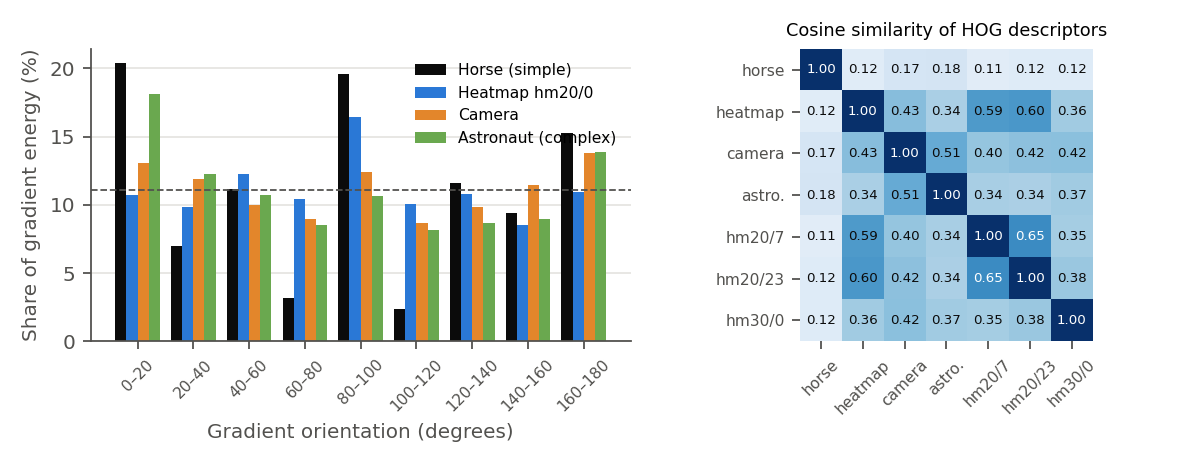
\includegraphics[width=\textwidth]{figurer/hog_sammenligning.png}
    \caption{Left: share of the gradient energy in each orientation bin; the dashed line is a uniform distribution. Right: cosine similarity between the full HOG descriptors, including two more participants on slide \texttt{hm20} and one participant on another slide (\texttt{hm30}).}
    \label{fig:hog-compare}
\end{figure}

The full descriptors keep the spatial layout, so the cosine similarity between two descriptors measures whether the same kind of edge appears in the same place (Figure~\ref{fig:hog-compare}, right). The mean similarity between the four different subjects is 0.29, and the horse is below 0.18 against all others because its flat cells are empty. Heatmaps of different participants on the same slide reach 0.59--0.65, since the slide text is identical and only the fixation blobs differ. A heatmap from another slide reaches only 0.36, which is lower than the similarity between the heatmap and the camera photograph (0.43). HOG therefore does not capture that two images are ``both heatmaps''. It compares cell by cell, and when the text lines are in different places, the cells no longer match. This spatial sensitivity is what makes HOG useful for detecting an object inside a fixed window, and it is also why it is unsuited to comparing whole scenes that are not aligned.

\emph{Effect of the parameters.}
Figure~\ref{fig:hog-params} shows how the cell size and the number of bins change the HOG image. In \texttt{skimage} the visualisation is drawn from the cell histograms before block normalisation, so the block size only affects the descriptor. To quantify the effects we vary one parameter at a time around the baseline and measure, averaged over the four images, the cosine similarity between each image and three modified copies: shifted by $(4,3)$ pixels, rotated $10^\circ$, and with the left half darkened to 10\% brightness. We also measure the mean similarity between the four different images, where a lower value means that the descriptor separates them better (Table~\ref{tab:hog-params}).

\begin{figure}[H]
    \centering
    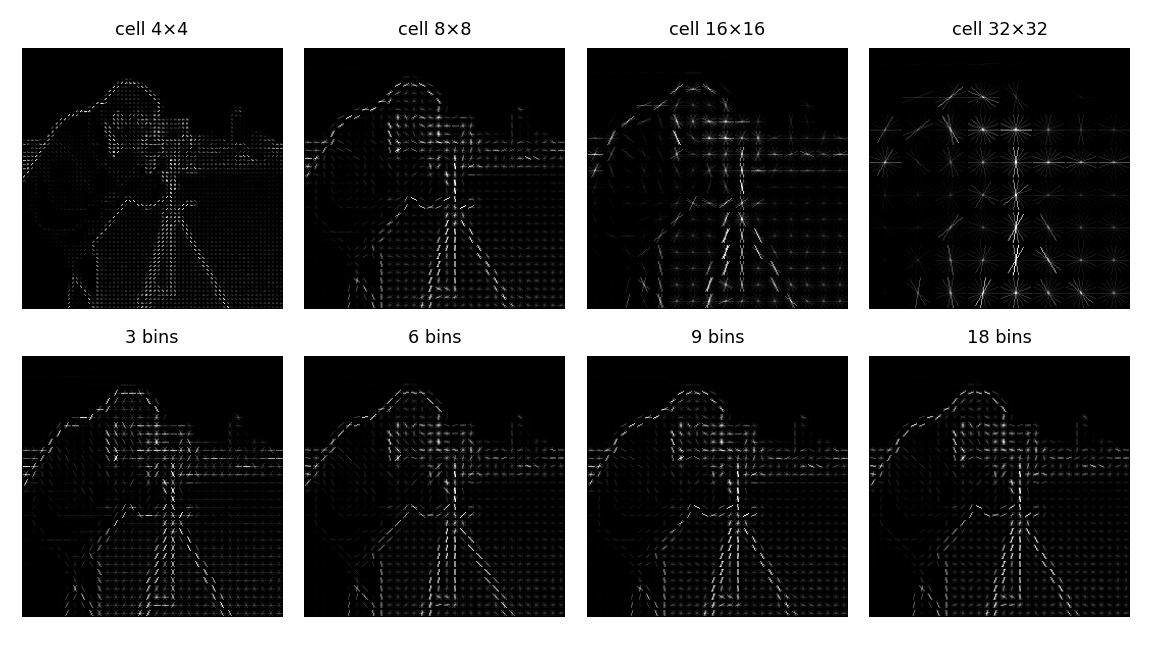
\includegraphics[width=\textwidth]{figurer/hog_parametre.png}
    \caption{HOG images of the camera image. Top: cell size 4 to 32 pixels (9 bins). Bottom: 3 to 18 bins ($8\times8$ cells).}
    \label{fig:hog-params}
\end{figure}

\begin{table}[H]
    \centering
    \begin{tabular}{llrrrrr}
        \toprule
        & & & \multicolumn{3}{c}{Similarity to modified copy} & Different \\
        \cmidrule(lr){4-6}
        Parameter & Value & Length & Shift & Rotation & Shadow & images \\
        \midrule
        Cell size & $4\times4$ & 142,884 & 0.50 & 0.34 & 0.83 & 0.21 \\
        (pixels) & $\mathbf{8\times8}$ & 34,596 & 0.72 & 0.46 & 0.89 & 0.29 \\
        & $16\times16$ & 8,100 & 0.87 & 0.63 & 0.93 & 0.39 \\
        & $32\times32$ & 1,764 & 0.96 & 0.80 & 0.95 & 0.53 \\
        \midrule
        Block size & $1\times1$ & 9,216 & 0.77 & 0.57 & 0.85 & 0.37 \\
        (cells) & $\mathbf{2\times2}$ & 34,596 & 0.72 & 0.46 & 0.89 & 0.29 \\
        & $3\times3$ & 72,900 & 0.71 & 0.41 & 0.91 & 0.25 \\
        & $4\times4$ & 121,104 & 0.70 & 0.38 & 0.91 & 0.22 \\
        \midrule
        Bins & 3 & 11,532 & 0.80 & 0.60 & 0.90 & 0.43 \\
        & 6 & 23,064 & 0.75 & 0.51 & 0.88 & 0.34 \\
        & \textbf{9} & 34,596 & 0.72 & 0.46 & 0.89 & 0.29 \\
        & 12 & 46,128 & 0.70 & 0.43 & 0.87 & 0.27 \\
        & 18 & 69,192 & 0.67 & 0.38 & 0.86 & 0.23 \\
        \bottomrule
    \end{tabular}
    \caption{Descriptor length and cosine similarity when one parameter is varied from the baseline (bold). Higher similarity to the modified copy means more robust; lower similarity between different images means more discriminative. Averages over the four images.}
    \label{tab:hog-params}
\end{table}

\emph{Cell size} has the largest effect. Small cells ($4\times4$) follow the individual edges, such as the tripod legs and the outline of the head, but the descriptor has 142,884 values, and a shift of only 4 pixels moves edges into neighbouring cells, so the similarity drops to 0.50. Large cells ($32\times32$) give a coarse summary: each star mixes many edges, the fine structure disappears, and the descriptor becomes nearly invariant to shift and rotation (0.96 and 0.80). It also becomes much less discriminative, since different images reach a similarity of 0.53. The cell size therefore sets the scale of the structures HOG describes, and it should roughly match the size of the parts that matter, which is why $8\times8$ suits a $64\times128$ pedestrian.

\emph{Block size} controls the region over which the contrast is normalised. Without any normalisation, the similarity to the shadowed copy is 0.78. With L2-Hys over $2\times2$ blocks it rises to 0.89, and to 0.91 with $4\times4$ blocks, because an edge in the dark half is scaled up to the same level as an edge in the bright half. Larger blocks also make the descriptor more discriminative (0.22), but each cell is repeated in up to $B^2$ blocks, so the length grows from 9,216 to 121,104, and the similarity after a rotation falls from 0.57 to 0.38. $1\times1$ blocks normalise each cell on its own, which can lift weak edges and noise in almost flat cells to the same level as strong edges.

\emph{Bins} set the angular resolution. With 3 bins, all orientations are forced into $60^\circ$ bins, so the curved edges in Figure~\ref{fig:hog-params} become angular, and the descriptor tolerates a $10^\circ$ rotation well (0.60) but separates the images poorly (0.43). With 18 bins the resolution is $10^\circ$, and a $10^\circ$ rotation moves most votes into a neighbouring bin, lowering the similarity to 0.38. The visual difference between 9 and 18 bins is small, while the length doubles, which agrees with Dalal and Triggs, who found little gain above 9 bins.

In summary, every parameter trades robustness against discrimination and descriptor length. Smaller cells, more bins and larger blocks give a longer and more discriminative descriptor that is more sensitive to small shifts and rotations. The baseline of 9 bins, $8\times8$ cells and $2\times2$ blocks is a compromise between the two.
